\chapter{INTRODUÇÃO}\label{cap:introducao}

Sistemas de segmentação de imagens têm se tornado populares em
variadas aplicações, como, por exemplo, a área de edição de imagem,
diagnósticos médicos e parte da visão computacional necessária pra
reconhecimento de objetos. Entre estes motivos e outros, essa área tem
uma relevância científica alta considerando a situação social,
tecnológica e econômica que é vivida no século XXI.\@

A segmentação de uma imagem pode ser feita manualmente por um anotador
humano marcando as linhas delineadoras de um objeto. Por outro lado,
são conhecido algoritmos variados para segmentação de imagens baseados
em aprendizagem de máquina.

Na Figura~\ref{fig:image-segmentation-types} é apresentado um quadro
comparativo de operações em uma imagem com balões, incluindo os tipos
de segmentação de imagens conhecidos: semântica e instância. Na
segmentação semântica o objetivo é segmentar apenas os mesmos tipos de
objetos como o mesmo rótulo, na segmentação por instância, cada balão
é visto como a mesma classe de balão por rótulos diferentes.

\begin{figure}[h!]
        \captionsetup{width=16cm}
		\Caption{\label{fig:image-segmentation-types}
Comparação de tipos de segmentação de imagem: por semântica e instância
}
		\centering
		\UFCfig{}{\fbox{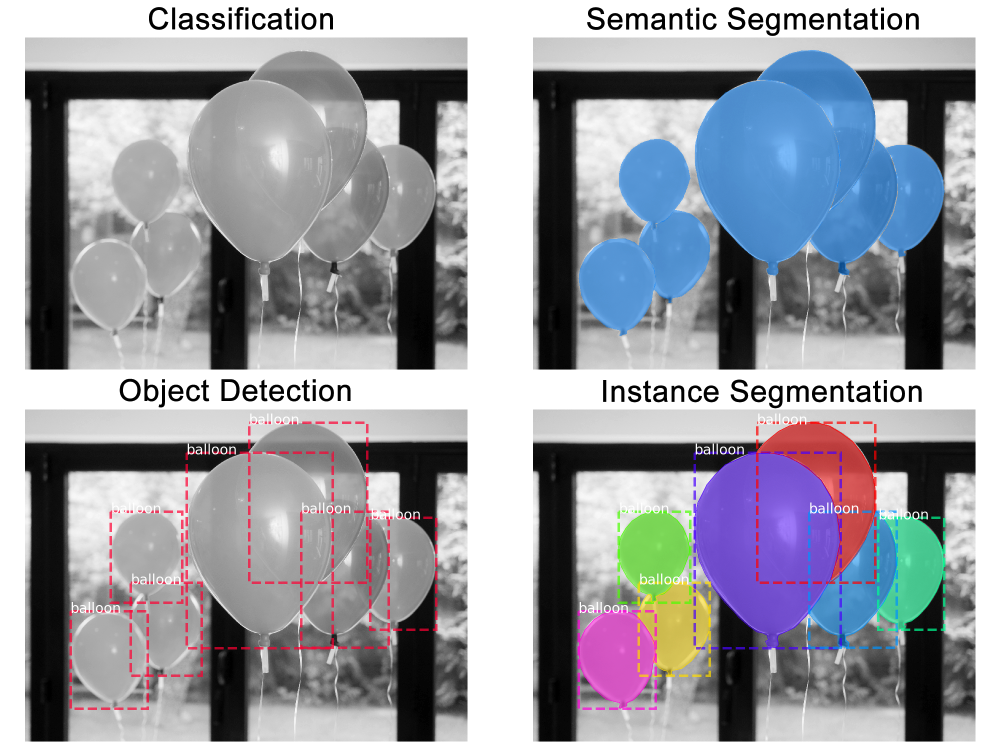
\includegraphics[width=16cm]{figuras/image-segmentation-types}}}{\Fonte{\citeonline{MediumInstanceSegmentation2019}}}
\end{figure}


Entre os tipos de aprendizagem de máquina, para segmentação de imagens
semântica é selecionada neste trabalho especificamente a aprendizagem
semi-supervisionada transdutiva (mais informações na seção~\ref{sec:teorica-aprendizado-semi-supervisionado}). A
aprendizagem semi-supervisionada é uma categoria que realiza o
aprendizado com poucas rotulações e maior parte dos dados não são
rotulados. Outras categorias de aprendizado de máquina como
supervisionada possui no treinamento uma base totalmente rotulada
enquanto a aprendizagem não-supervisionada não possui rótulo algum
(exemplo: K-means). Ao considerar a dificuldade de conseguir dados
rotulados por humanos em ambientes de uso especialistas, como imagens
médicas e ferramentas de edição de imagem, a abordagem
semi-supervisionada se demonstra interessante por necessitar de poucos
dados rotulados, mas ainda existir uma anotação com viés do
especialista interessado (médico, editor).


Os três principais algoritmos clássicos de segmentação de imagem podem
ser citados: \textit{Region-Based Segmentation}; \textit{Edge Detection
  Segmentation}; \textit{Segmentation based on Clustering}
~\cite{ImageSegmentationTechniques1985}. Cada uma dessas técnicas
possui limitações conhecidas, e entre elas é possível mencionar: haver
muitos objetos na imagem pode dificultar a segmentação; tempo
computacional elevado; sensibilidade ao contraste em escala cinza.

A abordagem estado da arte para segmentação de imagens
semi-supervisionada indutiva utiliza \gls{CNN}. A técnica é conhecida
como \textit{Mask R-CNN}~\cite{he2018mask}, funciona bem em casos
diversos e supera as técnicas anteriores nas métricas de segmentação,
mas possui ainda uma grande limitação: alto custo computacional para
treinamento da rede neural profunda e muitos dados anotados são
necessários.

Considerando tal situação-problema, este trabalho propõe a construção
de uma técnica de segmentação de imagem semi-supervisionada utilizando
redes complexas e dinâmicas coletivas de tal maneira que tenha menor
complexidade computacional em relação a \textit{Mask R-CNN} e seja
robusta em relação aos problemas enfrentados pelas técnicas clássicas.
